\subsection{Premi::Back-End}
	\subsubsection{Informazioni sul package}
		\begin{figure}[h]
			\centering
			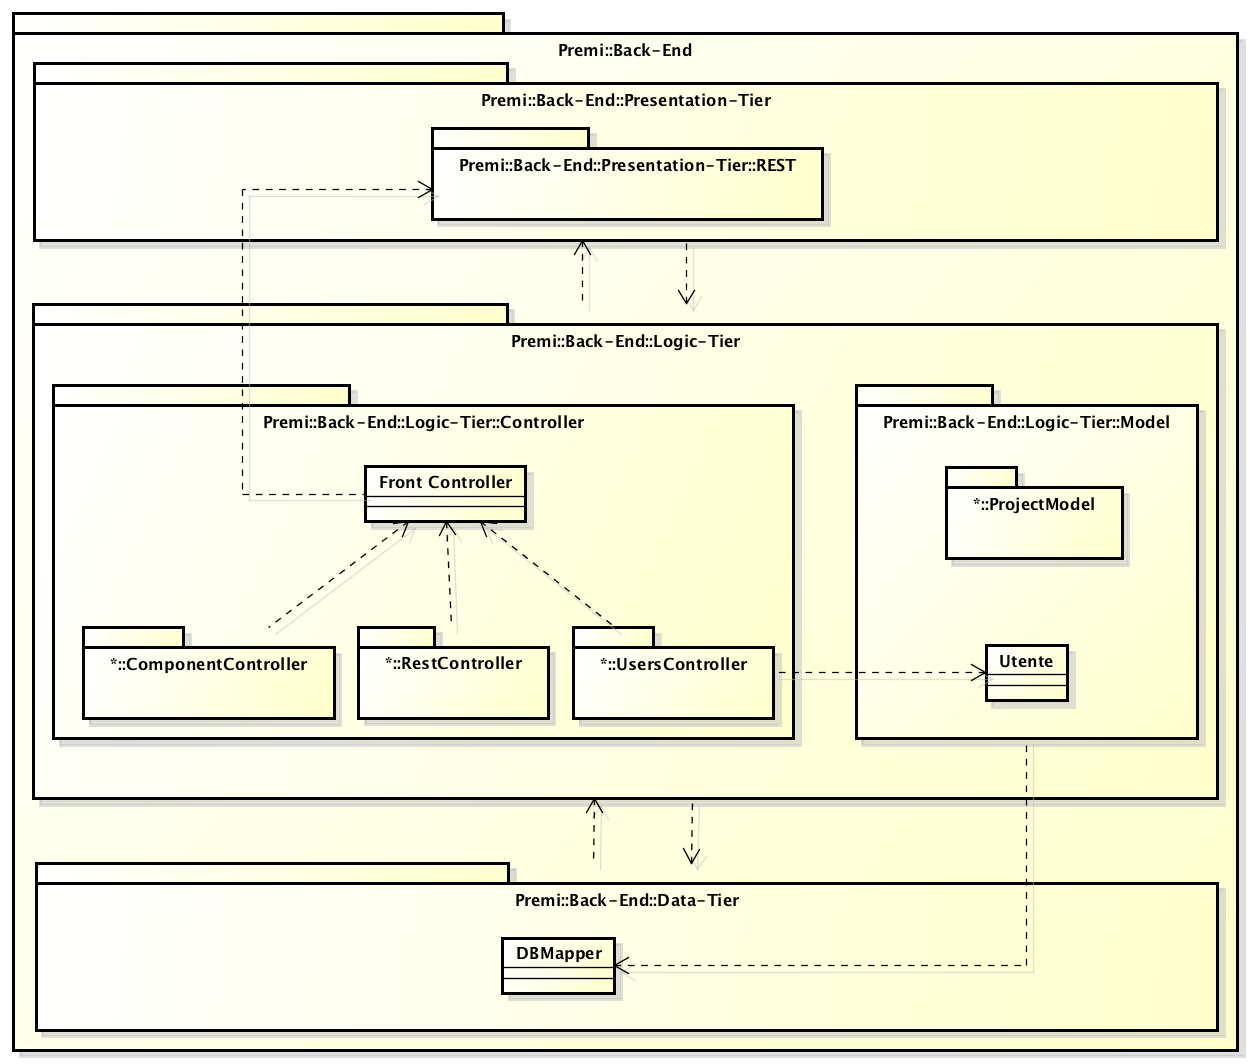
\includegraphics[width=\linewidth]{img/back-end-package}
			\caption[Premi::Back-End]{Premi::Back-End}
		\end{figure}
		Il package contiene le componenti della parte di back-end dell'applicazione.
		
	\subsubsection{Package contenuti}
		\begin{itemize}
			\item *::Presentation-Tier
			\item *::Logic-Tier
			\item *::Data-Tier
		\end{itemize}


\subsection{Premi::Back-End::Presentation-Tier}
	\subsubsection{Informazioni sul package}
		\begin{figure}[h]
			\centering
			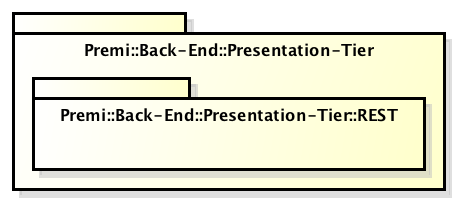
\includegraphics[width=0.5\linewidth]{img/back-end-package_presentation-tier}
			\caption[Premi::Back-End::Presentation-Tier]{Premi::Back-End::Presentation-Tier}
		\end{figure}
		Il package contiene le componenti necessarie per consentire il funzionamento del servizio REST, in modo tale da rendere possibile l'interfacciamento con il front-end.
		
	\subsubsection{Package contenuti}
		\begin{itemize}
			\item *::REST
			\begin{itemize}
				\item Descrizione: Il package contiene la struttura necessaria al funzionamento dell'architettura REST.
			\end{itemize}
		\end{itemize}
		
		
\subsection{Premi::Back-End::Logic-Tier}
	\subsubsection{Informazioni sul package}
	\begin{figure}[h]
		\centering
		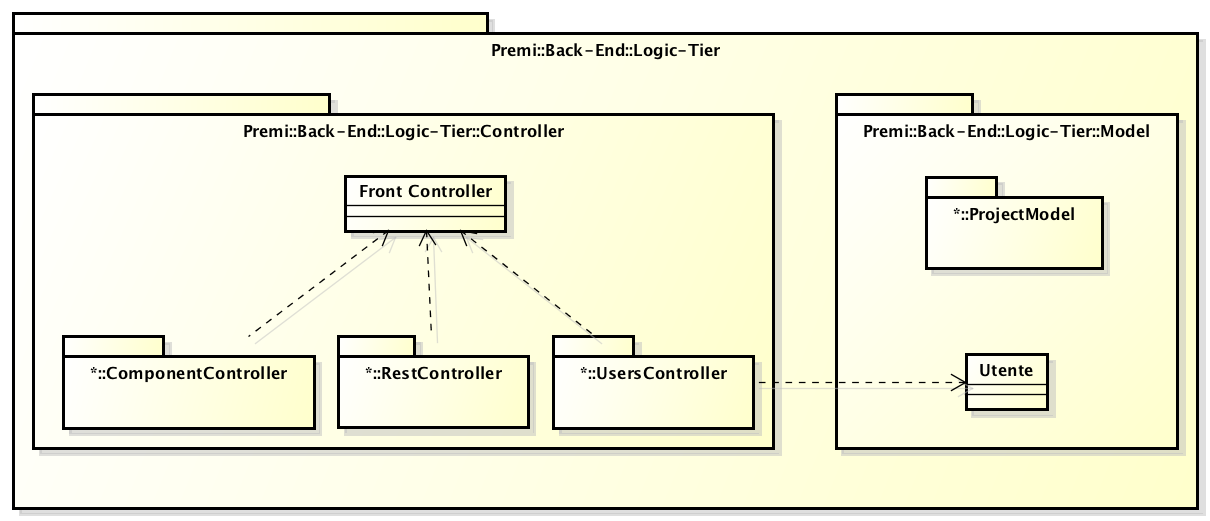
\includegraphics[width=0.7\linewidth]{img/back-end-package_logic-tier}
		\caption[Premi::Back-End::Logic-Tier]{Premi::Back-End::Logic-Tier}
	\end{figure}
	Il package contiene le componenti che si occupano di ricevere le richieste dal Presentation-Tier e di elaborarle attraverso il controller.
	
	\subsubsection{Package contenuti}
	\begin{itemize}
		\item *::Controller
		\item *::Model
	\end{itemize}
	
	
\subsection{Premi::Back-End::Logic-Tier::Controller}
	\subsubsection{Informazioni sul package}
	\begin{figure}[h]
		\centering
		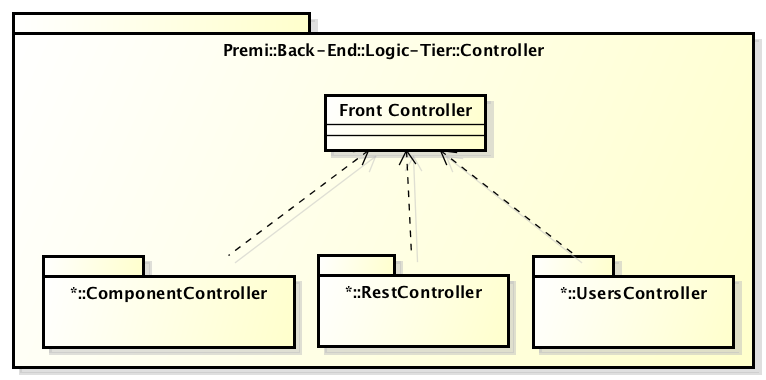
\includegraphics[width=0.7\linewidth]{img/back-end-package_controller}
		\caption[Premi::Back-End::Logic-Tier::Controller]{Premi::Back-End::Logic-Tier::Controller}
	\end{figure}
	Il package contiene le componenti che gestiscono la parte controller del lato back-end dell'applicazione. Al suo interno è presente l'interfaccia comune \textit{FrontController} dalla quale derivano tutti i controller del programma.
	Sono presenti i controller per il progetto e i suoi componenti.

\subsubsection{Package contenuti}
	\begin{itemize}
		\item *::ComponentController
		\begin{itemize}
			\item Descrizione: Il package contiene i controller per la gestione degli elementi di una slide.
		\end{itemize}
		
		\item *::RestController
		\begin{itemize}
			\item Descrizione: Il package contiene i controller per il REST.
		\end{itemize}
		
		\item *::UsersController
		\begin{itemize}
			\item Descrizione: Il package contiene gli elementi di controller per la gestione delle funzioni per l'utente, come login, registrazione, ricerca, ecc.
		\end{itemize}
	\end{itemize}


%\subsection{Premi::Back-End::Logic-Tier::Model}

\subsection{Premi::Back-End::Data-Tier}
	\subsubsection{Informazioni sul package}
	\begin{figure}[h]
		\centering
		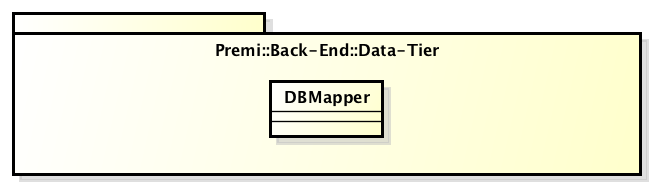
\includegraphics[width=0.5\linewidth]{img/back-end-package_data-tier}
		\caption[Premi::Back-End::Data-Tier]{Premi::Back-End::Data-Tier}
	\end{figure}
	Il package contiene le componenti che gestiscono l'interazione con il tier per la gestione dei dati consistenti. Fornisce un'interfaccia \textit{DBMapper} dalla quale derivano le classi in grado di elaborare le informazioni degli elementi dell'applicazione per poterli salvare nel database.